\typeout{NT FILE state-of-the-art.tex}

\prependtographicspath{{Chapters/Figures/}}

\chapter{State of the Art}
\label{cha:state-of-the-art}

In this chapter we'll explore how researchers have dealt with the challenges of creating an MAS based CPPS. We'll start by  examining the concepts of CPPS and MAS in more detail and by taking a look at the most commonly used designs and tools, as well as the recommended practices for an Industrial MAS. Finally, we'll do a brief analysis on some prototypes that were made to showcase the usefulness of an MAS in an industrial setting.

\section{Cyber-Physical Production Systems}
\label{sec:cyber-physical_production_systems}

As stated before, a Cyber-Physical System (CPS) is a system composed of two main entities, the physical system that contains all the hardware and resources and the cyber system that represents the physical system in the digital world. These two systems work together, the physical system sends data from the environment to the digital system and the digital system processes this data and instructs the physical system on what actions to perform. As such, this system works in a loop, constantly exchanging data and instructions to achieve a common goal.\\

A Cyber-Physical Production System (CPPS) is, as the name implies, a CPS that operates in a manufacturing setting. The physical system is composed of hardware like robot arms, Automated Guided Vehicles (AGVs), conveyor belts and specialized machinery for manufacturing. The cyber system might be as simple as a computer program or as complex as a full-on three dimensional model of the physical system. \citeauthor{birgit01} \cite{birgit01} proposed that a CPPS should:
\begin{itemize}
	\item Be service oriented, meaning that it should offer its services through the internet
	\item Be intelligent, with the ability to make decisions on its own
	\item Be interoperable, by having the capacity to aggregate and represent human-readable information and by providing a virtualization of the physical system
	\item Be able to flexibly adapt to changes in requirements and scale
	\item Have Big Data algorithm capable of processing data in real time
	\item Be capable of optimizing processes to increase Overall Equipment Effectiveness (OEE)
	\item Be able to integrate data across multiple disciplines and stages of the products life cycle
	\item Support secure communications to allow partnerships across companies
	\item Be capable of storing and accessing data in the Cloud
\end{itemize}

\section{Multi-Agent Systems}
\label{sec:multi-agent_systems}

%If I need more content I can probably expand this section

% Industrial Agents {paulo02}
To understand what should be the best practices in an MAS based CPPS, we first need to understand its base characteristics. A Multi-Agent System is, in essence a system composed by many entities called agents that have their own capabilities. These agents communicate and collaborate together by exchanging data among themselves and acting on that data to achieve a common goal. They are capable of adapting their behavior and of autonomous decision-making to determine the best course of action. This system is by nature decentralized and has no hierarchy, making it highly flexible and modular. At any point an agent can leave or join the system, without many changes in architecture \cite{paulo02}.\\

% Recommendation of Best Practices for Industrial Agent Systems based on the IEEE 2660.1 Standard {Leitao2021};
Industrial agents inherit all the qualities of software agents, like the intelligence, autonomy and cooperation abilities, but in addition are also designed to operate in industrial settings, and need to satisfy certain industrial requirements such as reliability, scalability, resilience, manageability, maintainability and most important of all, hardware integration \cite{Leitao2021}.\\

% Key directions for industrial agent based cyber-physical production systems {Karnouskos2019}
These requirements are generally tough to fulfill, especially so because despite the theoretical potential MAS have shown in supporting them, there aren't a lot of agent-based production systems outside the prototyping phase. This has stopped the growth of Industrial MAS due to the lack of practical knowledge in this field \cite{Karnouskos2019}. Another problem seen in Industrial MAS is the lack of models that can represent these systems. One of the key elements of an MAS are the changes made in structure and logic as the system operates. Thanks to the decentralized nature of the system, it is possible to add, remove or reconfigure modules freely to better adjust to the systems needs \cite{Karnouskos2019}.\\

Now that we have an idea of the characteristics and requirements for Industrial MAS, we can take a look at the most commonly used architectures, followed by what is recommended by the IEEE Standard.

\subsection{Best Practices and Common Architectures}
\label{subsec:best_practices_and_common_architectures}

% Integration patterns for interfacing software agents with industrial automation systems {8591641}
% IEEE Recommended Practice for Industrial Agents: Integration of Software Agents and Low-Level Automation Functions {9340089}
\citeauthor{Leitao2021} \cite{Leitao2021} analyzed the IEEE 2660.1 Standard for the recommended practices in integrating software agents and low-level automation functions. They described the use of an MAS as a CPPS, where control is decentralized, emerging from the interactions of agents that are part of the system. And as we've discussed before, one of the biggest problems is creating an interface between the agent and the device associated with it. Because of this, the IEEE 2660.1 Standard was created, defining the best practices in designing one an appropriate interface.\\

As an example, the authors mention three main types of interfaces. An interface for a smart sensor, to acquire measurements. An interface for a Programmable Logic Controller (PLC), to control simple devices like conveyor systems. And finally, an interface for a robot controller to control more complex functions in the CPPS. These three interfaces present different challenges on a development level, because each requires consideration on which architecture to follow, with different consequences to the evolution of the manufacturing plant over time.\\

The authors then created multiple scenarios, one of them being factory automation. They then proposed that the most valuable criterion was the response time of the system. As a secondary criterion scalability was chosen, but with a lesser importance. From this scenario the authors then concluded that a tightly coupled hybrid Open Platform Communications Unified Architecture (OPC UA) interface was preferable according to the IEEE 2660.1 standard. This means that the interface should have a client-server approach and be running remotely, a Tightly coupled Hybrid approach. However the authors also mention that this setup has a relatively low score, meaning that many of the other proposed practices are still viable, with testing needed to be done in order to pick the best one based on each specific scenario.\\


In \cite{Karnouskos2019}, it is proposed that one of the key requirements in the design of interfaces for MAS is interoperability. This comes with other challenges associated, like re-usability and scalability. In an MAS, the authors identified two main types of interfaces, the interface between agents, which normally is provided through the framework of the agent-based system, and the interface between agent and device. \\


\citeauthor{8591641} \cite{8591641} analyzed a study performed under the IEEE P2660.1 Working Group \cite{9340089} and concluded that most approaches followed a two-layer convention. The upper layer contained the agents part of the MAS and the lower layer the hardware associated with the physical production system. These two layers can interact in two ways \cite{8591641}:
\begin{itemize}
	\item Tight coupling, where the two layers communicate either through shared memory or through a direct network connection. This communication is synchronous and more direct.
	\item Loose coupling, where the two layers communicate through a queue or a pub/sub channel. This communication is asynchronous and less direct.
\end{itemize}

These layers can also be hosted in different setups \cite{8591641}:
\begin{itemize}
	\item Hybrid setup, where the two layers run in different devices.
	\item On-device setup, where the two layers run in the same device. 
\end{itemize}

This means that there can be four different interfaces, Tightly coupled Hybrid, Loosely coupled Hybrid, Tightly coupled On-device and Loosely coupled On-device.\\

A Tightly coupled Hybrid interface (Fig.~\ref{fig:tightly_coupled_hybrid}) is characterized by having the upper layer where the agent operates running remotely and accessing the lower layer through an Application Programming Interface (API). This API is responsible for translating the instructions given by the agent into commands the hardware can interpret. It is also responsible for the opposite, translating the hardware output, such as error codes or function results into data the agent can use. This approach is limited by the channel through which both layers communicate since both agent and device operate on two different computing platforms. This channel is affected by the amount of traffic in the network, more connections implies a lesser quality of service, namely in response time \cite{8591641}.\\

\begin{figure}[hbt!]
	\centering
	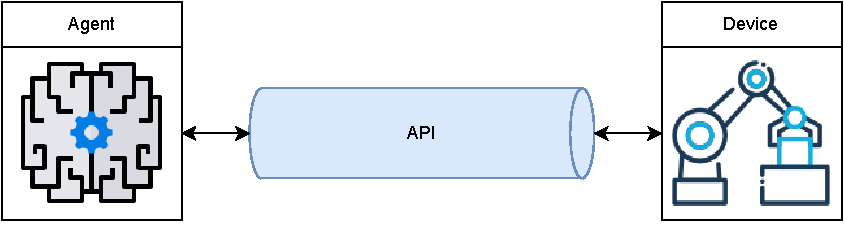
\includegraphics{TightlyCoupledHybrid}
	\caption{Tightly coupled Hybrid interface. Adapted from \cite{8591641}}
	\label{fig:tightly_coupled_hybrid}
\end{figure}

A Loosely coupled Hybrid interface (Fig.~\ref{fig:loosely_coupled_hybrid}) also sees both agent and device running on different computing entities. The difference is that instead of each agent having a direct connection to the corresponding device, they communicate through a message broker. Since the system still runs on two different computers it still suffers from the quality of the connection between layers, making this somewhat inappropriate for systems highly dependent on real time action. However, this approach sees better results in complex systems, where the agent layer needs to publish information to a large amount of devices at once. It also sees good results when it comes to scaling the system, since both layers are very independent of each other \cite{8591641}.\\

\begin{figure}[hbt!]
	\centering
	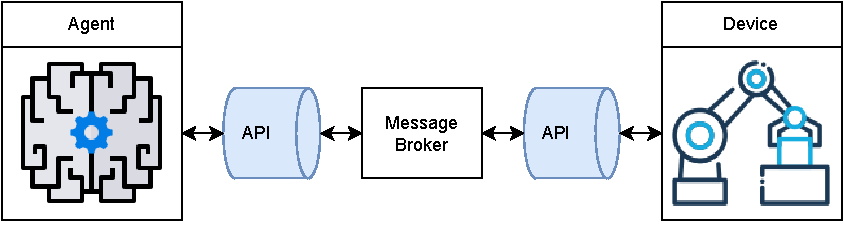
\includegraphics{LooselyCoupledHybrid}
	\caption{Loosely coupled Hybrid interface. Adapted from \cite{8591641}}
	\label{fig:loosely_coupled_hybrid}
\end{figure}

A Tightly coupled On-device interface (Fig.~\ref{fig:tightly_coupled_ondevice}) on the other hand follows an architecture where both devices share the same physical platform and can be done in two different ways. The first one, and far less common, has both agent code and device code compiled into a single binary running in the same computing element. This solution provides far better results in very demanding real time applications, however it also removes some flexibility from the system and is far more complicated to design due to the lack of development tools. The second option has the computational resources shared through a software library, where communication is done through software functions but abstracting some elements. This option still holds good results in real time control, but not as good as the first one \cite{8591641}.\\

\begin{figure}[hbt!]
	\centering
	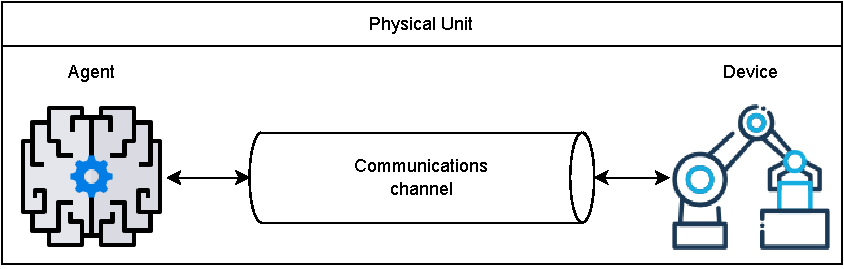
\includegraphics{TightlyCoupledOnDevice}
	\caption{Tightly coupled On-device interface. Adapted from \cite{8591641}}
	\label{fig:tightly_coupled_ondevice}
\end{figure}

Finally, a Loosely coupled On-device interface (Fig.~\ref{fig:loosely_coupled_ondevice}) is characterized by having the agent embedded in the device and communication is done through a broker. Both layers share a physical unit but do not share computational resources. The utilization of a broker between the two layers offers some flexibility, since the agent and hardware are less dependent of each other. This comes with the caveat that the real time response of the whole unit is dependent on the performance of the broker \cite{8591641}.\\

\begin{figure}[hbt!]
	\centering
	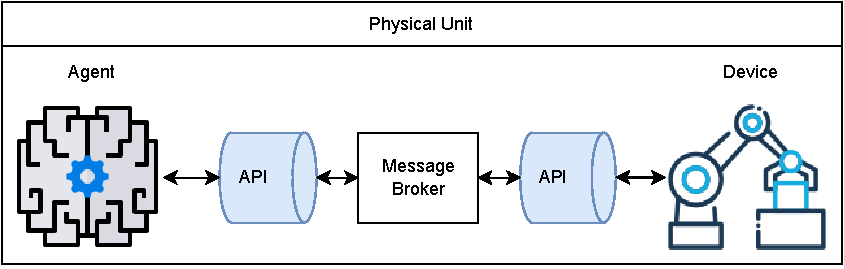
\includegraphics{LooselyCoupledOnDevice}
	\caption{Loosely coupled On-device interface. Adapted from \cite{8591641}}
	\label{fig:loosely_coupled_ondevice}
\end{figure}

%Talk about ROS?
The most common programming language to codify agents is Java, most likely due to JADE, an agent-based framework, followed by C++ \cite{8591641}. This framework helps developers in the implementation of MASs  with the FIPA specifications. It also allows deployment for different machines, due to Java supporting multiple devices \cite{JADE_website}.
For the device part, preexisting hardware is used in the majority of cases because it can be adapted into a MAS by using protocols such as OPC UA \cite{8591641}, which is a platform independent data exchange standard. It allows for both server-client and publish/subscribe communications \cite{OPCUA_website}.

% analysis on the specific interface implementations?
% I can probably analyze MAS with other objectives in mind to compare them to Industrial Agents?
\section{Practical Uses}

Adoption of industrial oriented MAS has been slow. According to \citeauthor{karnouskos02} \cite{karnouskos02}, the technology was still in its infancy almost two decades ago, with an incremental progress at best being made since then. In \cite{Karnouskos2019}, \citeauthor{Karnouskos2019} claim that agent-based applications in the industry is still limited. This is because despite the potential shown, these systems have not been implemented in real-world applications, where they would have the chance to evolve and leave the prototyping phase as new research is being done to make them more suitable for these applications.\\

There are, although, many research prototypes of MAS used for an industrial applications, and we'll take a look at some of them in this section.

\subsection{Bottling Plant}

%TODO add the other study conducted on this to expand this subsection

For the design of the bottling plant in \cite{bottling_plant_part2}, a research paper \cite{bottling_plant_part1} was first done by \citeauthor{bottling_plant_part2}, with the collaboration of multiple partners from different backgrounds. This was done to define the base requirements for project, which are:

\begin{itemize}
	\item Easy Scalability and Functional Expansion
	\item Manufacturer-neutral Resource Representation
	\item Robust Production Control by the Product
	\item Lot Size One without Identification
\end{itemize}

In addition to the requirements, \citeauthor{bottling_plant_part1} also designed a base solution approach. It consists of two generic agents, a Product Agent (PA) that represents individual products being manufactured, in this case the beverage bottles, and a Resource Agent (RA) that represents the resources used to manufacture the beverage bottles.\\

Since our main focus is on the interface between agent and hardware, we'll mainly focus on the RA. This agent must be generic in order to be implemented on multiple resources, so for each ResourceType there exists a ResourceConfig file which is loaded onto the RA in order to implement its interface. To give an example, if the resource has the ResourceType Machine, the ResourceConfig file MachineConfig must be read. The authors identified five different ResourceTypes and recognize that not all types have been considered. This means that for every new resource type that needs to be added to the system, a new ResourceConfig must be created in order to integrate the new RA into the system. In addition, a new resource that communicates differently from the ones already in the system would need a new interface, and thus a new ResourceConfig would also need to be created, even if the new resource performs similar functions in the manufacturing plant.\\

In \cite{bottling_plant_part2}, \citeauthor{bottling_plant_part2} created a service oriented bottling plant using the industrial agent system designed in \cite{bottling_plant_part1}, with positive results. To allow for extensibility of the system by additional resources a new agent class was created called InterfaceAgent (IntA). The ResourceConfig files for each type of RA now have a new field which contains an InterfaceAgentConfig. This new IntA is instantiated by the RAs following the configurations of their respective InterfaceAgentConfig and it extends either a DBLinkAgent, used to connect to a database, and a PLCLinkAgent, used to connect to a PLC UA client. All the information, like server address, port and authentication, is stored in the InterfaceAgentConfig file. By using OPC UA, the system can now interface with the hardware in the manufacturing plant, through a Loosely Coupled Hybrid interface. The authors recognize that according to the IEEE P2660.1 Working Group the scalability is considered weak, although they claim the flexibility is worth this loss in scalability.\\

To implement a new IntA, the following must be provided:
\begin{itemize}
	\item The communications protocol and the address, ports and authentication
	\item The way the interactions between the agent and resource should proceed
	\item The rules for the interpretation of internal resource states
\end{itemize}

Communication between the PLCLingAgent and the machine is done through simple commands that specify the type of program to use, depending on the size of the bottle, and the action to perform. However these commands need to be mapped to the manufacturer specific states through the PLCLinkAgent, making the system less scalable by default.\\

Nevertheless this system performed as intended, producing customized beverage bottles according the customers specifications.
 
\subsection{Agent-based Plug and Produce CPPS}

\citeauthor{8972169} \cite{8972169} have created a Plug and Produce CPPS. It is capable of integrating new agents on the fly, as the system operates. They accomplished this by having an agent detecting whenever a new agent joins the system or an existing one leaves. A java class was implemented using the Web Services 4 Devices - Java Multi Edition DPWS Stack (WS4D-JMEDS) framework, which searched for the devices in the network and obtained information about them. It was able to detect all devices connected to the network and add and remove them as needed.\\

This system was used to simulate a simple conveyor belt line with brushing capabilities. A product, represented by a PA enters the system and asks for the requisite action performed by sending a request to the FIPA Contract Net. All available agents then respond with their availability and the PA selects a Resource Agent to perform the action. If there is no RA available, either because all of them are occupied or there aren't any RAs with the capability to perform the action, the PA waits until one is available.
To test if the system can handle the dynamic movement of agents in and out of the system, some agents were disconnect from the network. The agent responsible for identifying changes in the network acted as expected, by removing agents that were no longer part of the network from the Contract Net, and by adding new agents to it.
This is a good example of a system capable of handling changes on the fly, without needing manual action for these changes to happen.\\

The MAS was developed using the JADE framework, the integration with the hardware done with Device Profile Web Services (DPWS). Whenever a physical action is needed by the system, the agent sends a SOAP message through DPWS to a PLC which in turn activates the corresponding action on the physical component. Although flexible and potentially scalable, this system still requires the individual programming of the PLCs according to the hardware they're integrated with.

\begin{figure}
	\centering
	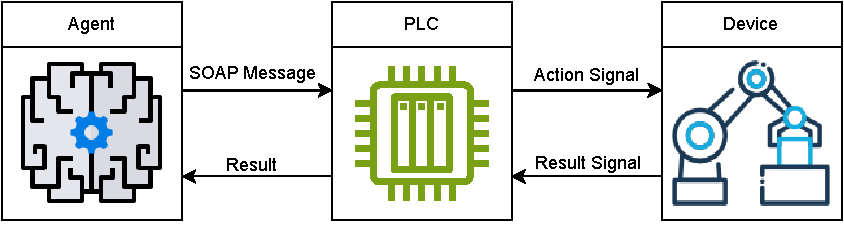
\includegraphics{PlugAndPlayDiagram}
	\caption{Plug and Produce Resource Agent. Adapted from \cite{8972169}}
	\label{fig:plug_and_play_device_architecture}
\end{figure}
%\subsection{Multi-agent Framework for Aircraft Parts}
%
%\citeauthor{6221793} \cite{6221793} created an MAS to manufacture aircraft structural parts. They were trying to optimize the manufacturing processes by integrating the agent-based approach in order to resolve bottlenecks in production. To accomplish this, many different types of agents were created:
%
%\begin{itemize}
%	\item A process planning agent to decide the appropriate tools for the current process.
%	\item A fixture design agent 
%\end{itemize}